\section{Visual Components for Data Analysis}

The AnyLogic simulation software provides a number of components for analysis of the simulation model. The list includes pie charts, bar charts, different plots and diagrams.

\begin{figure}[H]
  \centering
  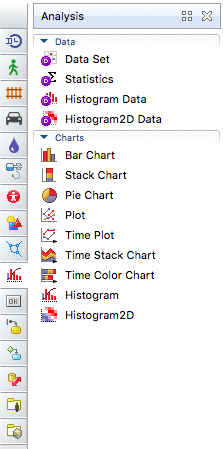
\includegraphics[height=0.5\textwidth]{img/screens/charts/charts1}
  \caption{The Analysis components for simulation model}
\end{figure}

We are going to add a time stack chart in order to see the dynamics of different populations in the model. As it can be seen from the figure, we added Susceptible, Resistant and Uncolonized values to the time stack chart. The system automatically deduces that the names refer to the values of corresponding stocks, which were created earlier.

\begin{figure}[H]
  \centering
  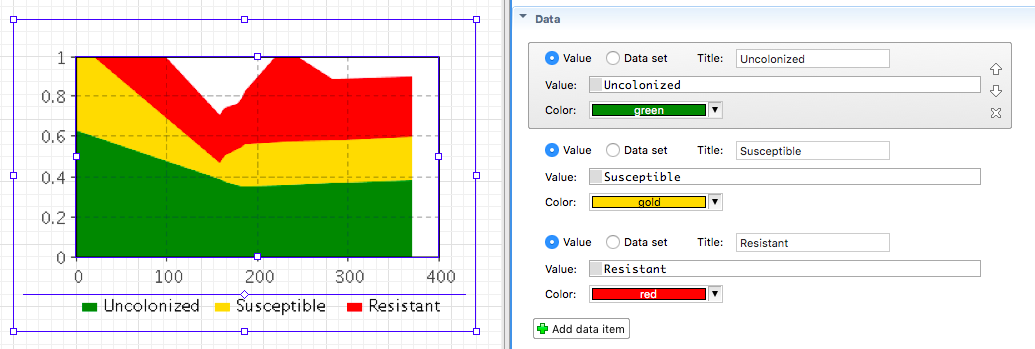
\includegraphics[width=0.8\textwidth]{img/screens/charts/charts5}
  \caption{The time stack chart for the observed groups}
\end{figure}

It is necessary to specify the scale of the time stack chart. Since we are observing the probabilities for an individual of falling into one of the three categories, we set the scale of the times stack chart to be from zero to one. This is because all of the probabilites should necessarily sum up to 1.

\begin{figure}[H]
  \centering
  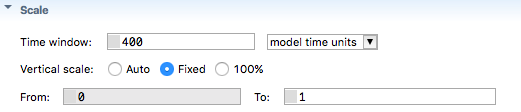
\includegraphics[height=0.2\textwidth]{img/screens/charts/charts3}
  \caption{The scale settings for time stack chart}
\end{figure}

We also set the data update settings of the time stack chart. Our chart will update the data automatically. We set it to display up to 400 last values of the stocks, since the width of the chart's "visible" area is equal to 400.

\begin{figure}[H]
  \centering
  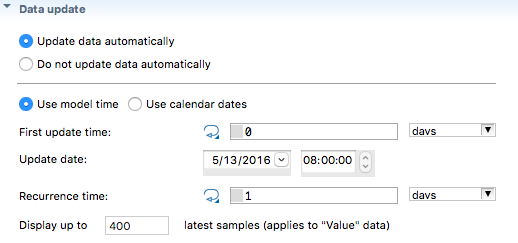
\includegraphics[height=0.3\textwidth]{img/screens/charts/charts4}
  \caption{Data update settings for the time stack chart}
\end{figure}